\section{Modeling}
\label{sec:modeling}

To test whether it is possible to prioritize PRs we have to model the data in such a way that an algorithm can learn and eventually predict what important pull requests are.

\subsection{Features}
\label{sec:features}

For creating a system that automatically creates an ordered list of PRs, we tried to use a machine algorithm that ranks the incoming PRs according to a set of features.
Most of the features we used (see table~\ref{tab:features}) are based on features that are used by many integrators to manually sort their PRs \cite{GZSD15}.

\begin{table*}[ht]
  \centering
  \begin{tabular}{rp{20em}rrrrc}
    \hline
    \textbf{Feature} & \textbf{Description} & \textbf{5\%} & \textbf{Mean} & \textbf{Median} & \textbf{95\%} & \textbf{Plot} \\
    \hline
    Age & Minutes between the moment the PR was opened and the current time. & 0.00 & 167344.02 & 77760.00 & 646560.00 & 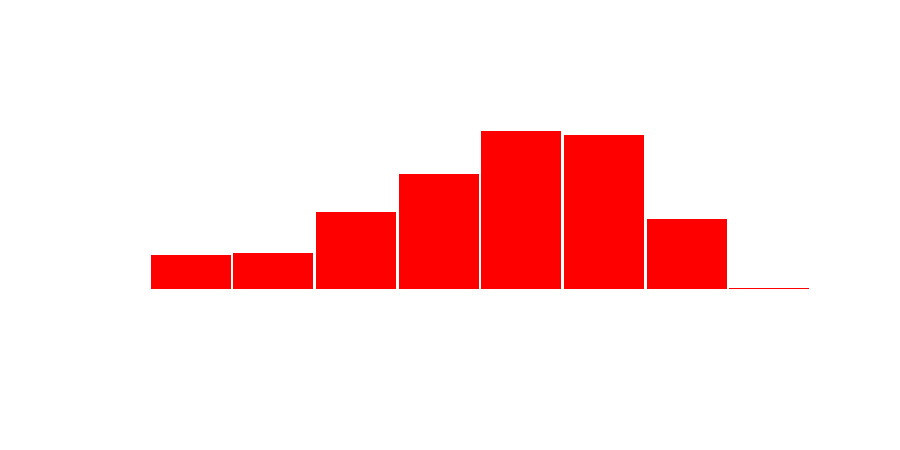
\includegraphics[scale = 0.1, clip = true, trim= 50px 60px 50px 60px]{../figs/hist-features/hist-age.pdf} \\
    Core Member & Boolean value indicating if the author of the PR is a project member. & 0.00 & 0.26 & 0.00 & 1.00 & 
\includegraphics[scale = 0.1, clip = true, trim= 50px 60px 50px 60px]{../figs/hist-features/hist-coreMember.pdf} \\
    Intra-Branch & Boolean value indicating if the PR originates and targets the same project. & 0.00 & 0.06 & 0.00 & 1.00 & 
\includegraphics[scale = 0.1, clip = true, trim= 50px 60px 50px 60px]{../figs/hist-features/hist-intraBranch.pdf} \\
    Contains Fix & Boolean value indicating if the pull request is a fix. & 0.00 & 0.18 & 0.00 & 1.00 & 
\includegraphics[scale = 0.1, clip = true, trim= 50px 60px 50px 60px]{../figs/hist-features/hist-containsFix.pdf} \\
    Contribution Rate & The percentage of commits already authored by the PR's author in the project. & 0.00 & 0.03 & 0.00 & 0.14 & 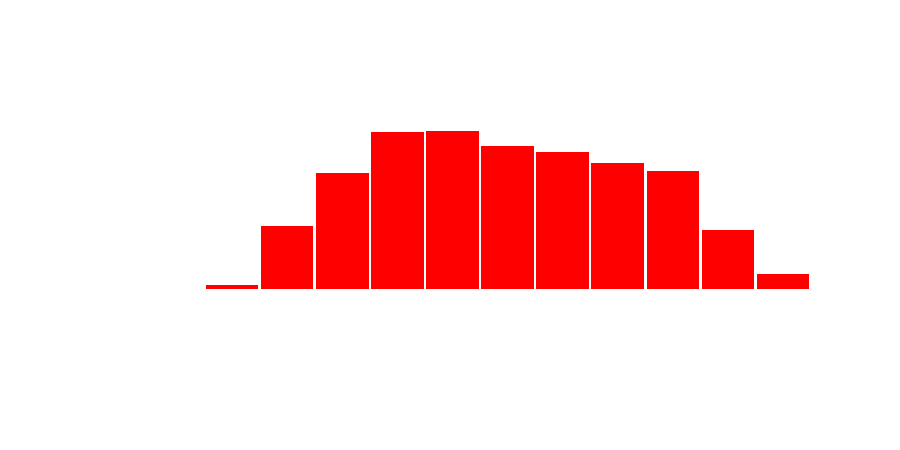
\includegraphics[scale = 0.1, clip = true, trim= 50px 60px 50px 60px]{../figs/hist-features/hist-commitRatio.pdf} \\
    Accept Rate & The percentage of the author's PRs that already have been merged. & 0.00 & 0.45 & 0.50 & 0.90 & 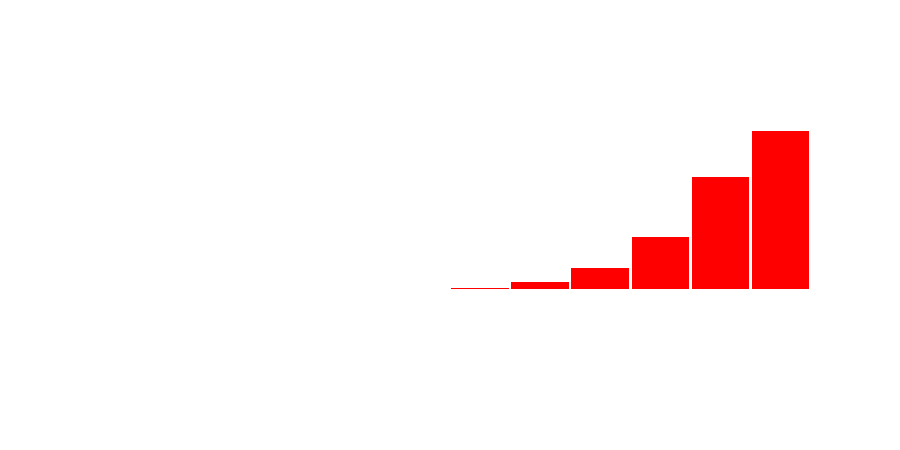
\includegraphics[scale = 0.1, clip = true, trim= 50px 60px 50px 60px]{../figs/hist-features/hist-pullRequestRatio.pdf} \\
    Comments & Number of discussion comments in the PR. & 0.00 & 4.22 & 1.00 & 17.00 & 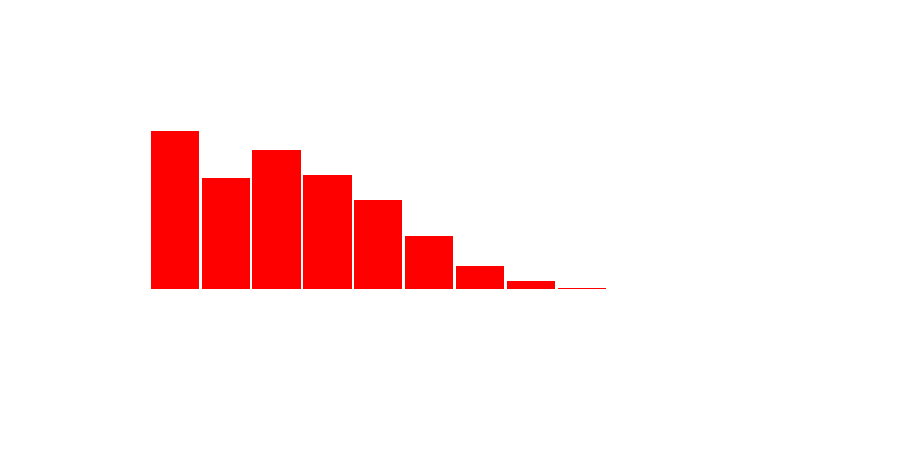
\includegraphics[scale = 0.1, clip = true, trim= 50px 60px 50px 60px]{../figs/hist-features/hist-comments.pdf} \\
    Review Comments & Number of code review comments in the PR. & 0.00 & 1.60 & 0.00 & 8.00 & 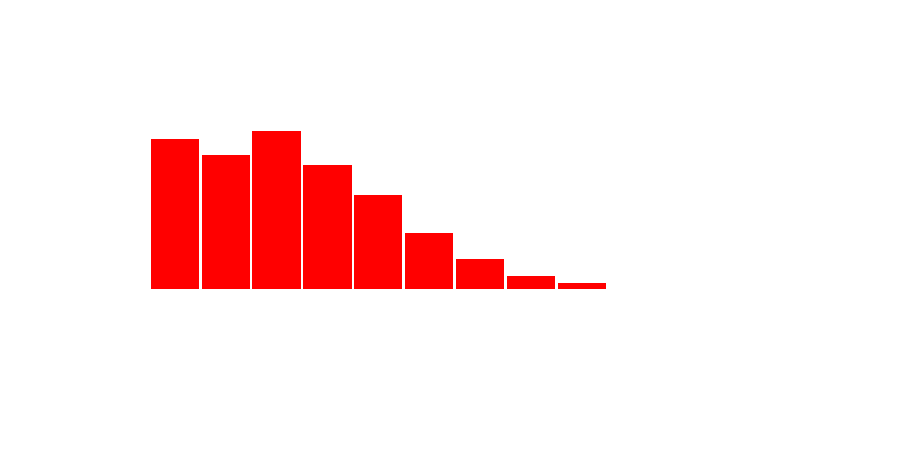
\includegraphics[scale = 0.1, clip = true, trim= 50px 60px 50px 60px]{../figs/hist-features/hist-reviewComments.pdf} \\
    Last Comment Mention & Boolean value indicating if the last comment of the PR contains a user mention. & 0.00 & 0.11 & 0.00 & 1.00 & 
\includegraphics[scale = 0.1, clip = true, trim= 50px 60px 50px 60px]{../figs/hist-features/hist-lastCommentMention.pdf} \\
    Additions & Number of lines added by the PR. & 1.00 & 3649.86 & 41.00 & 6285.00 & 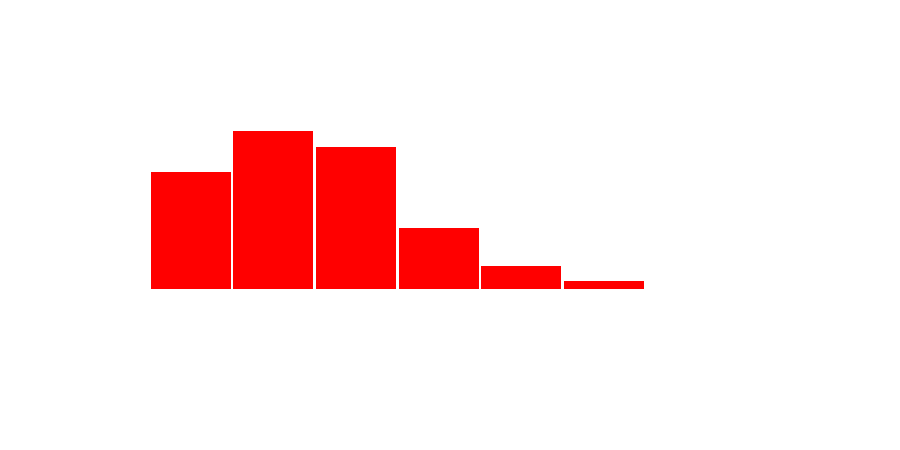
\includegraphics[scale = 0.1, clip = true, trim= 50px 60px 50px 60px]{../figs/hist-features/hist-additions.pdf} \\
    Deletions & Number of lines deleted by the PR. & 0.00 & 2271.32 & 7.00 & 2353.00 & 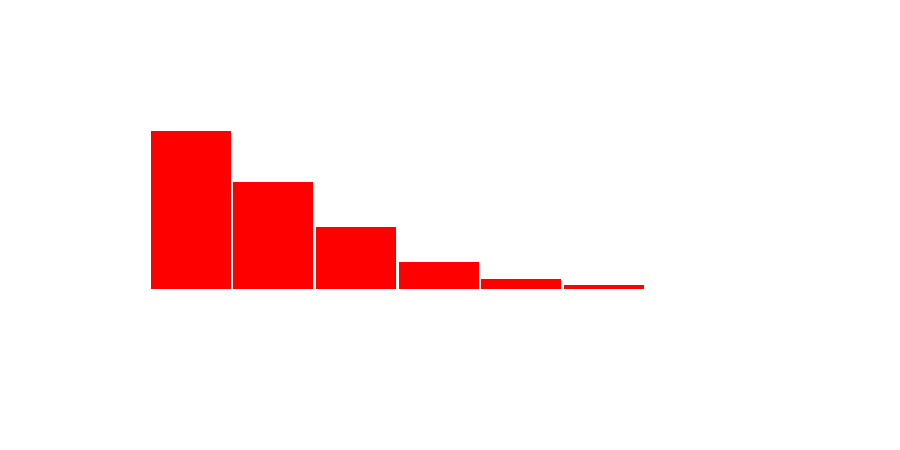
\includegraphics[scale = 0.1, clip = true, trim= 50px 60px 50px 60px]{../figs/hist-features/hist-deletions.pdf} \\
    Commits & Number of commits in the PR. & 1.00 & 6.52 & 2.00 & 22.00 & 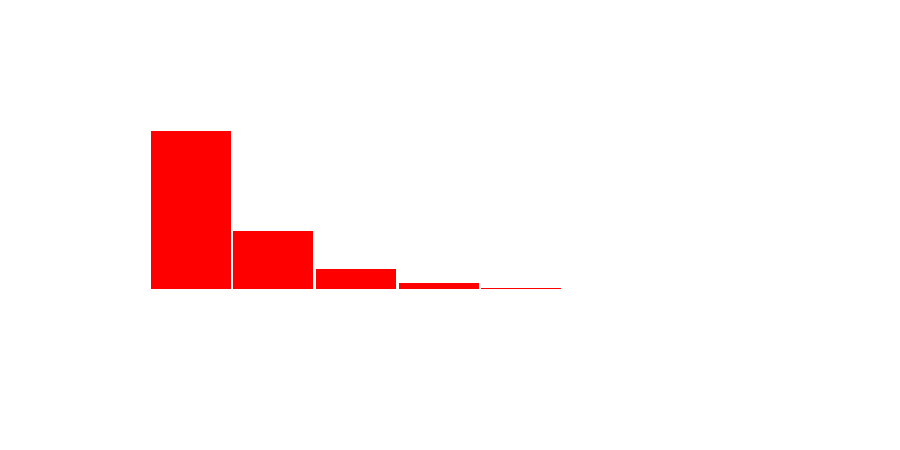
\includegraphics[scale = 0.1, clip = true, trim= 50px 60px 50px 60px]{../figs/hist-features/hist-commits.pdf} \\
    Files & Number of files touched by the PR. & 1.00 & 53.88 & 2.00 & 125.00 & 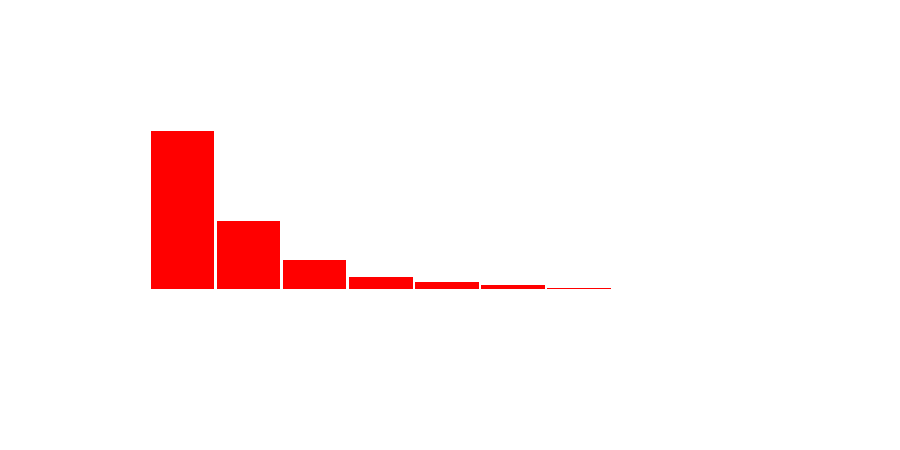
\includegraphics[scale = 0.1, clip = true, trim= 50px 60px 50px 60px]{../figs/hist-features/hist-files.pdf} \\
    Has Test Code & Boolean value indicating if tests are included by the PR. & 0.00 & 0.35 & 0.00 & 1.00 & 
\includegraphics[scale = 0.1, clip = true, trim= 50px 60px 50px 60px]{../figs/hist-features/hist-hasTestCode.pdf} \\
    \hline
  \end{tabular}
  \caption{Selected features and descriptive statistics. Histograms (red) are in log scale.}
  \label{tab:features}
\end{table*}

There is a very large group of integrators that take the PR's \emph{size} into account when manually prioritizing their PRs.
To capture this in our model we have four features (additions, deletions, commits, files) that depend on the size of the change.
The \emph{age} seems also a important feature when prioritizing PRs manually, so we included it in our model.
Also many integrators use the \emph{criticality of the fix}, \emph{urgency of feature} or \emph{type} of a PR as feature to prioritize.
It is difficult to measureme the criticality or urgency of a PR, instead we try to determine the type of a PR in a trivial way.
We define a boolean value indicating whether the pull request contains some sort of bug fix rather than e.g.\ a feature.
This is really just an indication as the value is only true if the PR contains the string ``fix'' in its title.
In general PRs with a fix are prioritized over other PRs.

The \emph{contributors track record} is also taken into account by integrators.
We have three features (core member, contribution rate, accept rate) regarding the track record of pull requesters.
The value of these feature may vary a lot between different projects.
There are integrators that look at PRs of known or trusted contributers first, their code is of known quality and often easier to review.
On the other hand there are also integrators that value PRs of new contributors more than those of known contributers.
The rationale behind this is that new contributers are feeling more valued when they receive a fast response on their PR.
Possibly will that feeling encourage them to continue to contribute to the project.
The accept rate feature suffers possibly from accuracy problems, as it is difficult to determine whether a PR is actually merged or not.
A pull request can be merged in different ways \cite{GPD14}.
Merges performed via the GitHub interface are easy to detect, but a PR which is squashed to one commit before it is merged is difficult to detect.

As second prioritization criteria the \emph{existence of tests} emerges as an important feature.
Some projects have a extensive test suite.
In these projects it is often expected that new PRs contain tests for the code they add.
The heuristic used for the test code detection is very trivial, the value of the feature is true if the PR changes at least one file with ``test'' or ``spec'' in its file name.

\subsection{Pairwise conflicts}
\label{sec:pairwise}

Some features we came up with are relevant for prioritizing, but are difficult too implement.
Therefore these features are not included in the training data, but they are available for manual sorting (see visualizer in section~\ref{sec:visualizer}).
\emph{Pairwise conflicts} is one of these features.

When the conflicts among other pending PRs are known, it can be used to determine a merge order in which the number of conflicts is reduced.
The actual number of conflicts is not reduced, but they can be concentrated in a particular merge action.
Figure~\ref{fig:conflicts-1} and \ref{fig:conflicts-3} show an example of the same set of three PRs but with different merge orders which result in a different amount of merge conflicts.
Pairwise conflicts are only checked among PRs which target the same branch, but nevertheless the amount of pairs can be very high.
In the worst case, i.e. when all PRs target the same branch, the number of pairs to be checked is $O(n^2)$.

Since checking the pairwise conflicts takes quadratic time it would take a large amount of time to create the training data which requires multiple time windows for each pull request (see section~\label{sec:training}).
It boils down to $O(n^2 \cdot m)$ where $m$ is the average number of time windows per PR.
Because of this time complexity, we decided to leave this feature out of the ML algorithm and only make it available for manual sorting.

\begin{figure}
  \centering
  % Trim option's parameter order: left bottom right top
  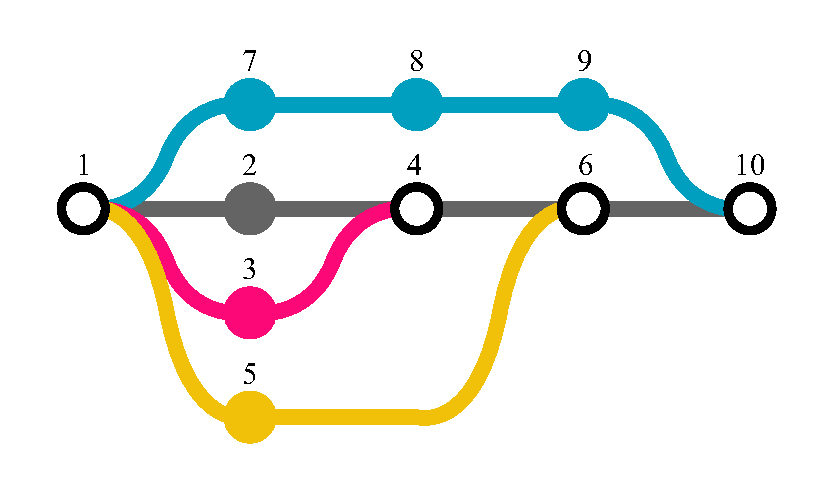
\includegraphics[height=25mm, clip ,trim = 0mm 7mm 0mm 7mm]{../figs/conflicts-1.pdf}
  \caption[Merge diagram with one conflict]
   {Merge diagram with one merge conflict.
   Consider the following conflicted commit pairs: $(2,7)$, $(3,8)$, $(5,9)$.
   The conflicts occur only in merge commit $10$.}
  \label{fig:conflicts-1}
\end{figure}

\begin{figure}
  \centering
  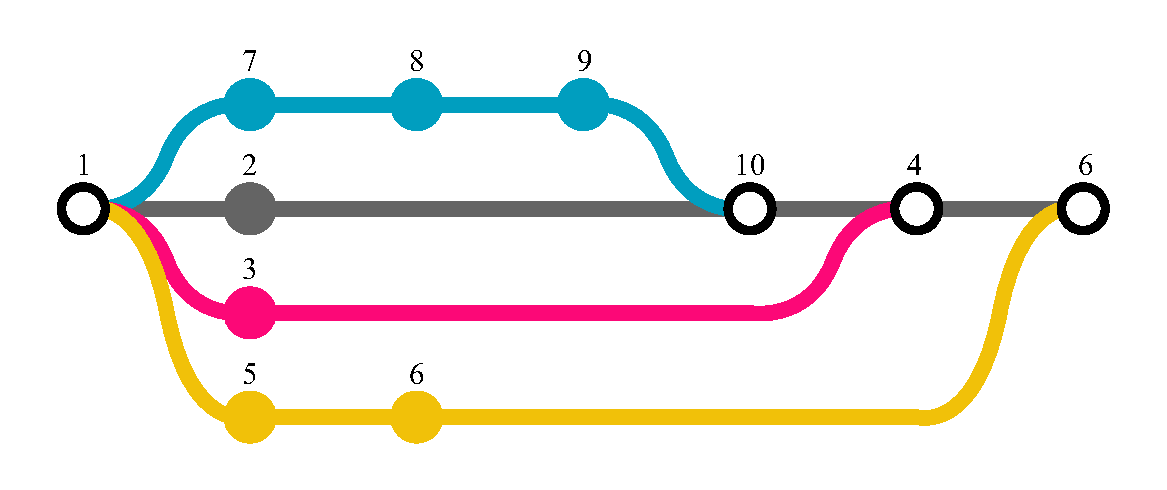
\includegraphics[height=25mm, clip ,trim = 0mm 7mm 0mm 7mm]{../figs/conflicts-3.pdf}
  \caption[Merge diagram with three merge conflicts]
   {Merge diagram with three merge conflicts.
   Consider the following conflicted commit pairs: $(2,7)$, $(3,8)$, $(5,9)$.
   The conflicts occur in each of the three merge commits $10,4,6$.}
  \label{fig:conflicts-3}
\end{figure}

\subsection{Training data}
\label{sec:training}

With the features described in the previous section we construct the training data.
For reasons discussed earlier we do not include the \emph{target branch} and \emph{pairwise conflicts} features.
There are different approaches of applying the pull-based development model \cite{GPD14}.
Because of this we create a different training set for every different GitHub project.

To train a prediction model so that it recognizes PRs that need attention, we have to provide it with actual examples of pull requests that we consider important.
We define important pull requests as follows: the current state of a pull request is important when an action follows on that PR.
An action can either be a merge, close, comment or review comment action.
To find out what the important states were, we have to dig into the past of previously closed PRs.
All the available information about the closed pull requests is extracted from \ghtorrent.
To determine the state of PRs in the past we take a systematic approach by dividing the lifetime of each PR into time windows.
The windows, with an interval of a day, contain a snapshot of the PR at the beginning of the window.
A PR's snapshot consists of its commits, comments and author info at the time.
Now that every PR is broken down into a list of consectutive snapshots, we can add information about the importance.
When an action is carried out within a certain time window, the snapshot contained in that window is marked as \emph{important}.
Snapshots of time windows that don't have any actions are not marked as important.
The final training data consists of these snapshots, where each snapshot is a row in the training data.
